\chapter{Performance Evaluation}
\label{chpt:experiments}

In this chapter, I will present experimental results on the performance of the
introduced parallel algorithms. First, we will take a look at the set-up of the
experiments and the environment (section~\ref{sec:experiments-set-up}), on which
they have been conducted. Then, we will consider the performance of stand-alone
parallel union-find (section~\ref{sec:experiments-union-find}) and afterwards
analyze the experimental results obtained for parallel area opening
(section~\ref{sec:experiments-area-opening}). In each section, I will introduce
the test data used and how it was generated, followed by a description, visual
presentation and discussion of the obtained results.

\section{Micro-benchmarks in Managed Languages}
\label{sec:experiments-microbenchmarks}

Proper performance measurements in managed languages, such as Java, are
difficult for various reasons. Java source code is compiled to byte code in
order to be executed by a JVM. The byte code is not optimized. The JVM uses
Just-in-Time (JIT) compilation and either interprets the byte code, or compiles
it when it deems this necessary \cite{Sestoft2013Microbenchmarks}.

In order to avoid spending time on compilation during the benchmark, the code is
usually executed a couple of times before the performance is actually
measured. Repeated execution triggers compilation of code, as it seems to the
JVM that certain functions need to be executed a lot and should therefore run
fast. Also, redundant code (e.g. a function's return value is never used) can be
optimized away by the JVM. Therefore, one needs to make sure that extremely high
performance of code is not related to the functions under test not being
executed at all \cite{Sestoft2013Microbenchmarks}.

In order to avoid costly JIT-compilation during performance measurement, the
micro-benchmark framework, which I developed for the experiments presented here,
executes each algorithm three times before starting measurements in its
respective configuration. Since union-find is an algorithm based on
side-effects, the JVM cannot determine, whether resulting values are unused and
therefore executes them.

Garbage collection is contained by calling \inlinecode{System.gc()} right before
the benchmark. Since this call is just a heuristic for the garbage collector, it
might not necessarily push all garbage collection outside of the benchmarked
sections. In order to handle variances in system-load and other factors, each
algorithm is executed ten times and the average duration (and other metrics) of
all ten executions is returned.

\section{Set-Up}
\label{sec:experiments-set-up}

The machine used for benchmarks runs on an \textit{AMD Opteron\texttrademark
  Processor 6386 SE} with 16 cores at 2800 megahertz
\cite{AmdOpteronSpecsWebsite}. The operating system is Ubuntu Linux 12.04 LTS
with kernel version~\textit{3.2.0-60-generic}. For the Java experiments, I used
OpenJDK, \textit{Java HotSpot\texttrademark} 64-Bit Server VM,
build~\textit{23.25-b01} with 2 gigabyte of memory assigned.

All processor-level metrics, like accumulated cache-misses, number of issued
instructions and the like, have been collected using \textit{perf}
\cite{PerfWiki} (version \emph{3.2.55}). The micro-benchmark framework starts
\emph{perf stat} anew from within the program for each run of the benchmarked
algorithm and only for the current process, so that exclusively events, which
occur during the benchmark, are recorded. Note that \emph{perf} is a Linux-only
tool.

All source code, as well as the resulting raw data and scripts required to
reproduce and display the results of this thesis, can be obtained at
\url{https://bitbucket.org/fbie/wait-free-morphology}.

\section{Union-Find}
\label{sec:experiments-union-find}

\subsection{Input Data}
\label{sec:experiments-uf-input-data}

The input data for parallel union-find benchmarks consists of graphs generated
with the graph generator package \emph{GTgraph} \cite{MadduriGTgraph}, which is
based on the \citet{Erdos1959Random} model. The \citet{Erdos1959Random} model
describes an undirected graph $G = (n, p)$ through a number of nodes $n$, and a
number $0 \leq p \leq 1$, which expresses the probability that any two nodes of
the graph are connected by an edge. In this model, $p$ can be seen as a measure
of connectivity of the graph. The input data has been generated in the same way
as by \citet{Berman2010Multicore}, in order to reproduce his results. The
experiments were conducted on four different input graphs. Two graphs for $n = 5
\cdot 10^5$ with $p = 10^{-6}$ (\emph{low-low}) and $p = 5\cdot 10^{-6}$
(\emph{low-high}) and additionally, two graphs for $n = 10^6$ with respective
probabilities $p = 5 \cdot 10^{-6}$ (\emph{high-low}) and $p = 10^{-5}$
(\emph{high-high}).

During benchmarking, the union-find data structure was initialized with $n$
nodes. Then, each thread was assigned a subset of the graph's edges, which were
represented by pairs of nodes, pseudo-randomly and called \inlinecode{union} on
each pair once. Each node in the graph is initially a singleton in the set of
disjoint sets \cite{Berman2010Multicore}.

\subsection{Results and Discussion}
\label{sec:experiments-uf-results}

The timing results of the union-find benchmark are depicted in
figure~\ref{fig:uf-results-ms}, where the duration for building the graph is
shown in milliseconds across the number of used hardware threads. The benchmark
results contradict the conclusions drawn by \citet{Berman2010Multicore}: the
optimistic, fine-grained locking algorithm (denoted \emph{optimistic})
outperforms the wait-free algorithm (\emph{wait-free}) only in the
\emph{low-low} case (see figure~\ref{fig:uf-results-ms-low-low}). Here,
\emph{optimistic} scales very nicely with the number of available hardware
threads. All other graph configurations with more nodes or higher connectivity,
force \emph{optimistic} to run very slowly in comparison to the other images
(figures~\ref{fig:uf-results-ms-low-high} through
\ref{fig:uf-results-ms-high-high}). The results for the various union-find
algorithms for the latter cases are very similar. I will therefore focus on the
analysis of the results shown in figure~\ref{fig:uf-results-ms-low-low} and
\ref{fig:uf-results-ms-low-high} in the following.

\begin{figure}
  \centering
  \unionfindplotlow{ms}
  \unionfindplothigh{ms}
  \caption[Execution time for parallel union-find in milliseconds.]{Execution
    time for parallel union-find in milliseconds. Note, how the performance of
    \emph{optimistic} degrades with increasing connectivity of the input graph.}
  \label{fig:uf-results-ms}
\end{figure}

\begin{figure}
  \centering
  \unionfindplotlow{retries}
  \caption[Number of union-find retries.]{Number of union-find retries. The
    recorded values are the number of STM-retries and the number of
    re-executions of the while-loop for \emph{optimistic} and
    \emph{wait-free}. The increase of retries is modest for increased
    connectivity.}
  \label{fig:uf-results-retries}

  \unionfindplotlow{cache-misses}
  \caption[Cache misses for parallel union-find.]{Cache misses for parallel
    union-find. The recorded metrics are very similar in both cases, which
    suggests that cache-misses are not the reason for the exhibited performance
    drop.}
  \label{fig:uf-results-cache-misses}

  \unionfindplotlow{instructions}
  \caption[Number of issued CPU instructions for parallel union-find.]{Number of
    issued CPU instructions for parallel union-find. Note, how the number of
    instructions increases nearly exponentially in the case of
    \emph{low-high}. Furthermore, note the different scale.}
  \label{fig:uf-results-instructions}
\end{figure}

\subsubsection{Analysis}

To find the reason for this behavior, we need to investigate other metrics as
well. Figure~\ref{fig:uf-results-retries} shows the number of times the root
nodes have become child nodes during \inlinecode{union}. Recall that this can
happen between locking two root nodes or between finding roots in a wait-free
fashion and then trying to unite them (see chapter~\ref{chpt:union-find}). In
the case of the STM variants (denoted as \emph{stm} and \emph{stm-while} for the
while-loop STM variant), the number of transactional retries were counted. The
curves for \emph{optimistic} are stable across both cases (compare
figures~\ref{fig:uf-results-retries-low-low} and
\ref{fig:uf-results-retries-low-high}) and do not exhibit any major, non-linear
increase. Note, that the retries under \emph{wait-free} and \emph{stm} are
slightly and irregularly increasing.

In figure~\ref{fig:uf-results-cache-misses}, we see the amount of accumulated
cache misses during the benchmark. In the optimistic case, there is a slight
increase of cache misses measurable (compare
figures~\ref{fig:uf-results-cache-misses-low-low} and
\ref{fig:uf-results-cache-misses-low-high}), but not to any extent that would
explain such a dramatic performance drop. Also, the STM variants both
consistently encounter cache misses that are roughly two orders of magnitude
higher than for \emph{optimistic}. If neither re-tries, nor cache misses are
responsible for the performance loss, it is reasonable to hypothesize that the
reason must simply be high lock contention due to higher connectivity of the
graph and therefore fewer disjoint sets.

The number of CPU instructions issued during benchmarking, as displayed in
figure~\ref{fig:uf-results-instructions}, confirms this hypothesis. In case of
\emph{wait-free}, \emph{stm} and \emph{stm-while}, the instructions stay roughly
constant across the used number of hardware threads and also across input
graphs. This is not the case for the optimistic algorithm (compare
figures~\ref{fig:uf-results-instructions-low-low} and
\ref{fig:uf-results-instructions-low-high}, note the different scale). The
executed instructions increase nearly quadratically, which hints at intense
spinning when waiting for a lock to become acquirable.

To understand, why increasing the probability by a factor of five has that much
influence on the performance, we need to look at the number of connected
components in the graph. According to the \citet{Erdos1959Random} model, the
number of connected components is dependent on $np$. If $np < 1$, then, with a
probability close to 1, no component will be larger than $O(log(n))$. If $np >
1$, then, with equal probability, there will be a giant connected component with
a size of at least $O(n^{2 / 3})$ \cite{Erdos1959Random, Erdos1960On,
  Bollobas1984Evolution}.

Since for \emph{low-low}, we have $(5 \cdot 10^5)(10^{-6}) = 0.5$, and $(5 \cdot
10^5)(5 \cdot 10^{-6}) = 2.5$ for \emph{low-high}, the latter is likely to
introduce a giant connected component to the graph. Since in optimistic
union-find, all elements of a connected component share the same root, we
encounter high lock contention when adding further vertices to the giant
connected component.

Other than that, it becomes clear that re-trying transactions is very
costly. The performance of \emph{stm} compared to \emph{stm-while} is not only
significantly slower but also less stable. Figure~\ref{fig:uf-results-retries}
shows not a single re-try for \emph{stm-while} is recorded. It is very likely
that this is due to \emph{multiverse} spawning new threads for every transaction
internally. Thereby, more software threads than hardware threads are run,
directly influencing performance negatively. Conflicts are results of
indeterministic thread scheduling. The more threads need to be scheduled, the
more potential conflicts to handle and the more new threads are spawned.

Conclusively, it seems that the optimistic algorithm is suitable for graphs of
low connectivity and that the performance of the pure STM algorithm is very
unreliable. Both these conclusions are not very encouraging with regard to image
analysis. One would, of course, like to run image analysis algorithms that
exhibit good performance, no matter the structure of the input, and also to
enjoy stable performance running the same algorithm on the same input twice.

\section{Area Opening}
\label{sec:experiments-area-opening}

\subsection{Input Data}
\label{sec:experiments-ao-input-data}

The input data for performance experiments on area opening are, of course,
images. We have to distinguish between two kinds of images, namely synthetic
images and natural images. Synthetic images are images generated by a computer
program (either programatically or manually). Natural images are images obtained
through cameras.

For the experiments presented here, synthetic images were used. Synthetic images
yield the advantage that one can benchmark the algorithms in a very controlled
manner and that it is easy to model extreme cases. The images are each of $1600
\times 1200$ pixels size each. They were generated using \emph{GNU Gimp} and
model five extreme case, displayed in figure~\ref{fig:synth}. The extreme cases
are chosen not only to asses the performance of the parallel algorithms
systematically, but also to verify a number of hypotheses.

\begin{figure}
  \centering

  \makebox[\textwidth][c]{
    \begin{subfigure}{0.3\textwidth}
      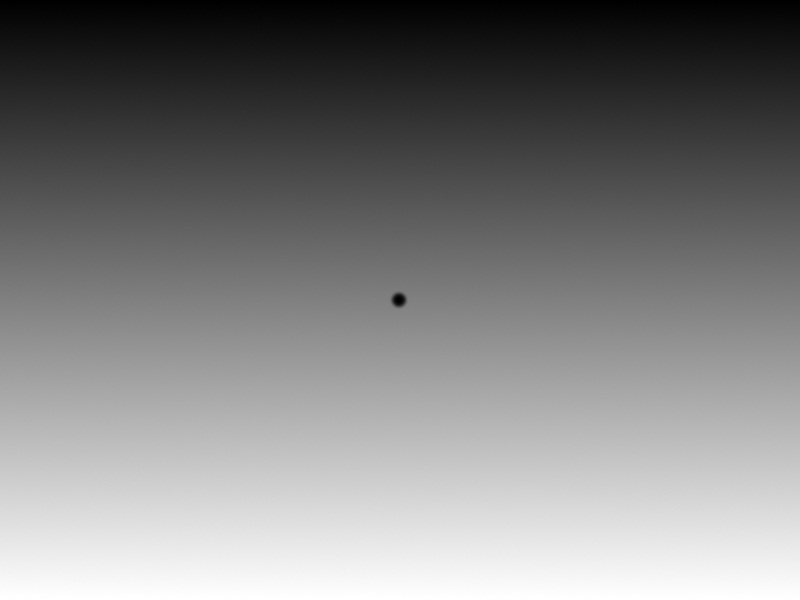
\includegraphics[width=\textwidth]{../data/synth001.jpg}
      \caption{Vertical gray-scale gradient (\emph{grad-vert}).}
      \label{fig:synth-a}
    \end{subfigure}
    ~~
    \begin{subfigure}{0.3\textwidth}
      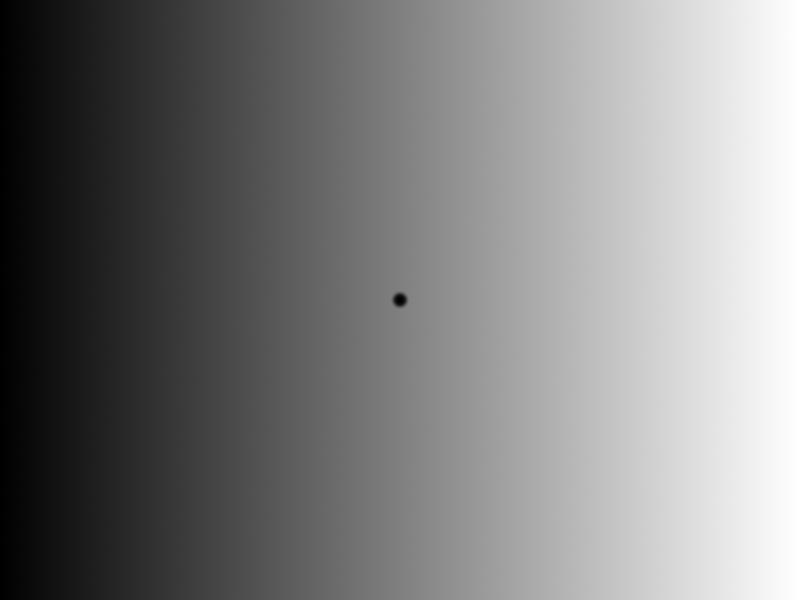
\includegraphics[width=\textwidth]{../data/synth002.jpg}
      \caption{Horizontal gray-scale gradient (\emph{grad-hrz}).}
      \label{fig:synth-b}
    \end{subfigure}
    ~~
    \begin{subfigure}{0.3\textwidth}
      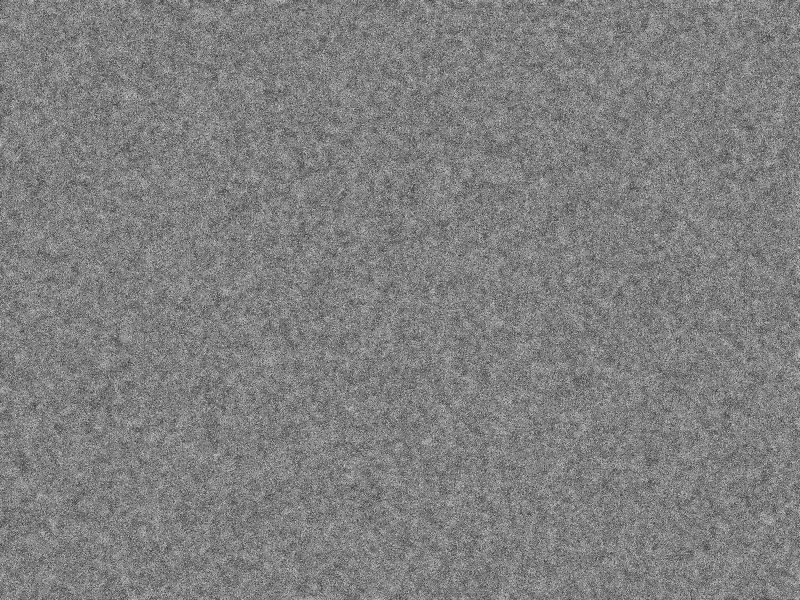
\includegraphics[width=\textwidth]{../data/synth003.jpg}
      \caption{Fine grained noise (\emph{noise-fine}).}
      \label{fig:synth-c}
    \end{subfigure}
  } % makebox

  \makebox[\textwidth][c]{
    \begin{subfigure}{0.3\textwidth}
      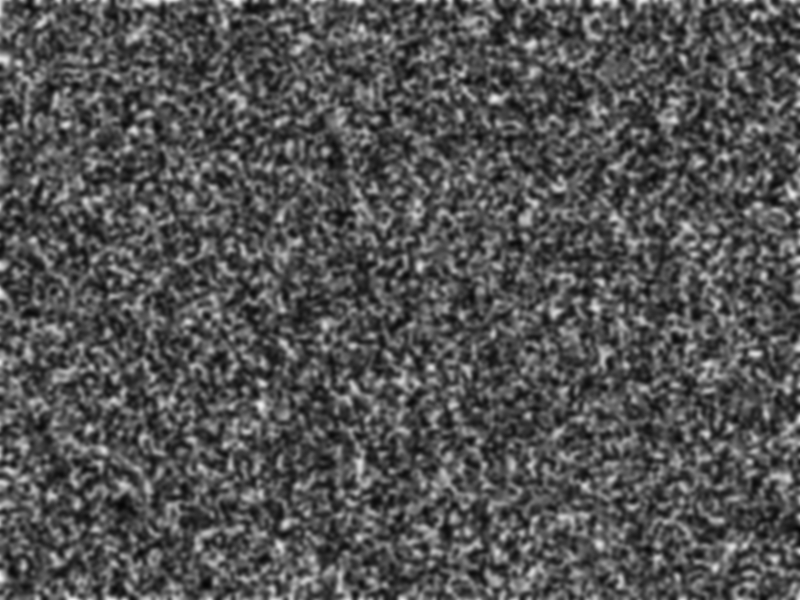
\includegraphics[width=\textwidth]{../data/synth004.jpg}
      \caption{Coarse grained noise (\emph{noise-coarse}).}
      \label{fig:synth-d}
    \end{subfigure}
    ~~
    \begin{subfigure}{0.3\textwidth}
      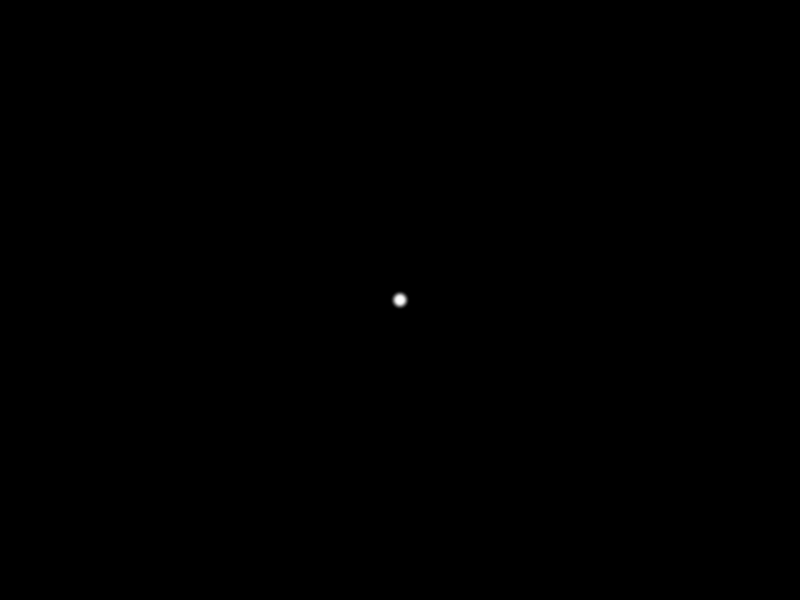
\includegraphics[width=\textwidth]{../data/synth005.jpg}
      \caption{Flat black component (\emph{flat}).}
      \label{fig:synth-e}
    \end{subfigure}
  } % makebox

  \caption[Synthetic input images for area-opening experiments.]{Synthetic input
    images for area-opening experiments. Each image models an extreme case of
    gray-scale image structure.}
  \label{fig:synth}
\end{figure}

\paragraph{Hypothesis 1}

The vertical gradient image in figure~\ref{fig:synth-a} (\emph{grad-vert}) is
supposed to force the sub-image filtering algorithms to work sequentially when
scanning pixels from light to dark. Each thread has to wait until the global
level pointer reaches the level that is within the threads pixel range. While
figure~\ref{fig:synth-b} also consists of a gradient from black to white, the
gradient direction is rotated by 90\degree (\emph{grad-hrz}). The hypothesis is
that sub-image filtering on \emph{grad-vert} is slower than on \emph{grad-hrz},
because there is no expected starvation for the latter, and that, overall,
\emph{grad-vert} is the worst-case for sub-image algorithms. Furthermore, one
can assume that filtering by lines outperforms sub-image filtering in this case.

\paragraph{Hypothesis 2}

Figures~\ref{fig:synth-c} (\emph{noise-fine}) and \ref{fig:synth-d}
(\emph{noise-coarse}) show images generated from random white noise to which a
Gaussian filter has been applied. The granularity of the noise differs, in order
to vary the size of the connected components in the image. We can expect high
performance on both \emph{noise-fine} and \emph{noise-coarse}, since the initial
connectivity is low, when the images are seen as graphs where each pixel is
definitely connected to its neighbors through an edge if the two pixels are at
the same gray level.

\paragraph{Hypothesis 3}

Finally, figure~\ref{fig:synth-e} (\emph{flat}) shows a single, major level
component and therefore has an extremely high connectivity. Based on the results
from section~\ref{sec:experiments-uf-results}, we can expect high contention for
each algorithm, since nearly all pixels are part of the same flat component.

\begin{figure}
  \centering
  \fullmsrow{\synthone}{hypothesis-1-a}
  \caption[Execution time in milliseconds for \emph{grad-vert}.]{Execution time in
    milliseconds for \emph{grad-vert}. In both cases, the performance of sub-image
    filtering algorithms is stable across number of threads.}
  \label{fig:hypothesis-1-a}

  \fullmsrow{\synthtwo}{hypothesis-1-b}
  \caption[Execution time in milliseconds for \emph{grad-hrz}.]{Execution time
    in milliseconds for \emph{grad-hrz}. The optimistic algorithms scale
    negatively with the number of threads, while the STM algorithms remain
    unstable in performance.}
  \label{fig:hypothesis-1-b}

  \fullmsrow{\synththreea}{hypothesis-2-a}
  \caption[Execution time in milliseconds for \emph{noise-fine}.]{Execution time
    in milliseconds for \emph{noise-fine}. The optimistic sub-image filtering
    algorithms improve over the sequential baseline. The STM algorithms run very
    slow in comparison.}
  \label{fig:hypothesis-2-a}
\end{figure}

\begin{figure}[t]
  \centering
  \fullmsrow{\synthfour}{hypothesis-2-b}
  \caption[Execution time in milliseconds for \emph{noise-coarse}.]{Execution
    time in milliseconds for \emph{noise-coarse}. The performance is comparable
    to \emph{noise-fine}.}
  \label{fig:hypothesis-2-b}

  \fullmsrow{\synthfive}{hypothesis-3}
  \caption[Execution time in milliseconds for \emph{flat}.]{Execution time in
    milliseconds for \emph{flat}. The optimistic sub-image filtering algorithms
    outperform the sequential algorithm. Still, the STM algorithms do not come
    close to the sequential baseline.}
  \label{fig:hypothesis-3}
\end{figure}

\subsection{Results and Discussion}
\label{sec:experiments-ao-results}

\subsubsection{Notation and Data Selection}

In this section, I will systematically analyze the results from benchmarking the
different area opening algorithms, based on the hypotheses from
section~\ref{sec:experiments-ao-input-data}. The figures reference the various
algorithms according to table~\ref{tab:algorithms-acronyms}. The only operation
measured is the main-loop of the algorithms. Again, the resolving step is
omitted entirely, mainly because the parallel resolving step would be the same
for all parallel algorithms. For brevity, I will not show and discuss the entire
hypercube of experiments and configurations, and instead present selected
results based on their relevance. After all, we face sixteen different
algorithms -- the algorithms use not only two different variants of shared
union-find, but also different sorting algorithms or shared queues -- and five
different images.

The raw data shows very similar results for \emph{block-counting} and
\emph{block-bucket}, as well as \emph{line-queues-msq} and
\emph{line-queues-array}, respectively, regardless of the underlying data
structures. Therefore, only one configuration of each of these algorithm pairs
is depicted in this section. The raw benchmark results for all algorithms can be
found in appendix~\ref{chpt:omitted-data}. The different queue implementations
only exhibit different performance in the case of \emph{pixel-queues-msq} and
\emph{pixel-queues-array}, which we will discuss in detail in
section~\ref{sec:experiments-ao-results-pixels}.

In this section, the optimistic, fine-grained union-find algorithm is denoted
\emph{opt}, while the STM variant is simply denoted \emph{stm}. If an algorithm
uses any of those algorithms, it is prepended by the according union-find
acronym.

The execution times for all synthetic images and for $\lambda = 3000$ are
shown in figures~\ref{fig:hypothesis-1-a} through \ref{fig:hypothesis-3}. In the
left column, we can see the performance of the optimistic union-find variant,
while on the right, the STM variant's performance is depicted. The legend holds
for each plot of the same column.

\subsubsection{Analysis}

When comparing the performance of optimistic and STM algorithms, it becomes
clear that the STM variants are systematically slower than the optimistic
implementations. This suggests that for practical values of $\lambda$, the
connectivity of the image is not high enough to provoke as much contention as
exhibited in the experiments from section~\ref{sec:experiments-uf-results}. Not
only this, but their performance is developing much more unstable over the
number of hardware threads. This is especially explicit in
figures~\ref{fig:hypothesis-2-a} and \ref{fig:hypothesis-2-b}. None of the STM
variants comes close to the performance baseline of the sequential
algorithm. Because of this obvious infeasibility of the STM algorithms (and for
brevity), I will focus on the analysis of those algorithms that use optimistic
union-find.

\paragraph{Hypothesis 1}

\begin{figure}
  \centering
  \plotrow{\synthone\retries\opt}{Retries for \emph{grad-vert}.}{analysis-hypothesis-1-a}{\synthtwo\cache\opt}{Cache misses for \emph{grad-hrz}.}{analysis-hypothesis-1-b}
  \caption[Performance metrics for \emph{grad-vert} and \emph{grad-hrz}
  (optimistic).]{Performance metrics for \emph{grad-vert} and \emph{grad-hrz}
    (optimistic). The amount of re-tries for sub-image filtering algorithms on
    \emph{grad-vert} is zero, as they are forced to work sequentially. The
    number of cache-misses does not reveal any insights into the negatively
    scaling performance on \emph{grad-hrz}.}
  \label{fig:analysis-hypothesis-1}
\end{figure}

The results, depicted in figure~\ref{fig:hypothesis-1-a}, support the initial
hypothesis that \emph{grad-vert} forces sub-image filtering algorithms to work
in a sequential fashion. The performance of those algorithms is stable over the
number of threads. There are two more observations that require further
analysis.

Firstly, \emph{line-queues-msq} is slower than the already to sequential
performance forced sub-image algorithms. Since the pixel-lines are shared
between threads, the algorithm should encounter less starvation, and therefore
perform faster. The decline in performance is actually due to contention, as we
can see in figure~\ref{fig:analysis-hypothesis-1-a} and due to increased cache
misses (not displayed). Because the threads work sequentially, when performing
sub-image filtering, there is nearly no lock contention on the union-find
roots. In contrast, line-by-line filtering encounters contention already with
only a few threads, as the threads are able to make progress in parallel.

Another interesting observation is that the performance of shared sorting
(\emph{block-counting}) is poor in every exhibited case. This is either due to
contention during sorting, due to starvation when iterating over the shared list
of pixels or even because of conflicts during uniting
pixels. Figure~\ref{fig:analysis-hypothesis-1-a} suggests that the latter is a
major factor.

Secondly, the performance on \emph{grad-hrz} scales negatively with the number
of threads. This is surprising, because the horizontal gradient should provoke
much less starvation than \emph{grad-vert}. The recorded metrics show a linear
increase of cache misses for all algorithms over the number of threads (see
figure~\ref{fig:analysis-hypothesis-1-b}). This alone does not explain the
performance decrease. We will get back to this behavior later in the text.

The hypothesis can only be confirmed partially: \emph{grad-vert} forces
sequential performance as expected, but \emph{grad-hrz} shows decreasing
performance for increasing number of threads. Also, line-based algorithms do not
provide better stability on vertical gradient images.

\paragraph{Hypothesis 2}

Figure~\ref{fig:hypothesis-2-a} and \ref{fig:hypothesis-2-b} support the
hypothesis that, for irregularly structured images, sub-image filter algorithms
excel in performance. Unfortunately, this is still not the case for STM
variants. Again, we can see that the overhead of maintaining single pixel-lines
does not pay off.

The sub-image filter algorithms and the pixel-line based algorithms scale nicely
with the number of threads. Their performance scales effectively up to around
eight threads, from where on no further substantial improvement is visible.

In these cases, even the shared sorting algorithms scale with the number of
available hardware threads. Nevertheless, their performance is still way below
the sequential baseline. We can also see that the STM variants scale according
to the number of threads, but their performance remains unstable and the plots
contain nearly no useful information. However, the hypothesis can be confirmed.

\paragraph{Hypothesis 3}

\begin{figure}
  \centering
  \plotrow{\synthfive\retries\opt}{Number of retries.}{analysis-hypothesis-3-a}{\synthfive\instructions\opt}{Number of issued CPU instructions.}{analysis-hypothesis-3-b}
  \caption[Performance metrics for \emph{flat} (optimistic).]{Performance
    metrics for \emph{flat} (optimistic). The performance of the shared sorting
    algorithm is influenced to a large degree by re-tries and lock contention.}
  \label{fig:analysis-hypothesis-3}
\end{figure}

When filtering a giant connected component, we ought to face high contention, as
shown by the results obtained in
section~\ref{sec:experiments-uf-results}. Surprisingly, the results shown in
figure~\ref{fig:hypothesis-3} show only a serious performance decrease for
\emph{block-counting}. The metrics displayed in
figure~\ref{fig:analysis-hypothesis-3} show that the number of instructions
increases nearly linearly with the number of hardware threads, while the number
of retries is consistently high.

On the other hand, the sequential and sub-image filtering algorithms excel in
this case. The pixel-line based algorithm does not show any performance
increase, but also no decline. The giant connected component seems not to have
any effect on the performance, which is comparable to the optimal case
(i.e. \emph{noise-fine} and \emph{noise-coarse}). This is surprising, as it
directly contradicts the notion that large connected components cause
contention. Neither the number of retries, nor the number of issued instructions
increases to any noticeable degree.

This suggests that there is few overlap between the single threads when
filtering sub-images. The starting indices of the independent threads are
located ``far away'' from each other (recall the sub-image filtering algorithms
described in sections~\ref{sec:area-opening-no-sorting-sub-image} and
\ref{sec:area-opening-local-sorting-sub-image}). Therefore, increased contention
only becomes an issue very late in the filtering process, as soon as threads
begin to unite connected components across sub-image borders. Since this is only
a small fraction of work compared to building the thread-local connected
components, its impact on the performance is minimal.

The hypothesis holds for some of the parallel area opening algorithms but cannot
be confirmed completely. The structure of the sub-image filtering algorithms
counters the effect of a giant connected component. This also suggests an
explanation for why the performance on \emph{grad-hrz} was unexpectedly
bad for sub-image filtering: since the level components on
\emph{grad-hrz} are ordered horizontally and extend across all sub-image
borders, contention is encountered very early, as each thread repeatedly tries
to unite its connected component with those of other threads already in the
beginning, so that all threads work on the same connected component, which is
therefore locked frequently.

\subsection{Pixel Queues}
\label{sec:experiments-ao-results-pixels}

\begin{figure}
  \centering
  \areaopenplotpixels
  \caption[Benchmark results for \emph{pixel-queue} variants on
  \emph{noise-coarse}.]{Benchmark results for \emph{pixel-queue} variants on
    \emph{noise-coarse}. The execution time is extremely high for each
    variant. The sequential performance baseline is barely visible.}
  \label{fig:pixel-queues}
\end{figure}

The results for pixel queue algorithms are special in terms of performance and
therefore, I devote a separate section to those. Figure~\ref{fig:pixel-queues}
displays the benchmark metrics for experiments on image \emph{noise-coarse}. For
the experiments, the image has been scaled down to $800 \times 600$ pixels, in
order to reduce the overall testing time. We can see from
figure~\ref{fig:pixel-queues-ms} that the performance of \emph{all} variants of
\emph{pixel-queues} is dramatically worse, especially with regard to the number
of hardware threads, than the base-line performance of the sequential algorithm.

Even though we can expect slow performance because of the missing sorting of
pixels, the results are surprising. The naive sub-image filtering algorithm,
which also operates in $O(kn)$, exceeds the sequential algorithm in
performance. Executing \emph{pixel-queues} algorithms, as described in
section~\ref{sec:experiments-microbenchmarks}, on a single image took in
practice about a day for all combinations of parameters. It is especially
interesting to investigate the reasons for this.

Here, both union-find variants behave very similarly for all metrics. We can
therefore already conclude that this is not a union-find based problem. Instead,
the different queue implementations seem to suffer heavily from high
throughput. The conflicts handled by the union-find implementations do not
increase together with the elapsed measured time. Therefore, even though
union-find conflicts might be responsible for the initial increase, they are not
the reason for the overall dramatic performance.

Instead, each queue data structure suffers from a different
phenomenon. Figure~\ref{fig:pixel-queues-cache-misses} shows how the number of
cache misses increases already when using only two threads for the bounded array
queue, probably due to false sharing \cite{Bolosky1993False}. False sharing
describes an effect caused by cache coherence protocols on shared memory
processors. Each processor has its own cache, which contains copies of the data
of the other processors' caches. When a processor writes a word into one of the
cache lines of its local cache, the entire cache line gets invalidated for all
other processors. Consequently, all other caches need to update this line. This
happens especially often, if more than one independent word is stored per cache
line, so that many words are falsely invalidated \cite{Bolosky1993False}. In
many cases, this invalidation would be unnecessary and it therefore results in a
slow down of the processors \cite{Bolosky1993False}. Notice how the shape of the
plot for the bounded array queue in figure~\ref{fig:pixel-queues-cache-misses}
resembles the one in figure~\ref{fig:pixel-queues-ms}.

The \citet{Anderson1994Waitfree} queue exhibits no false sharing. The reason for
its poor performance is depicted in
figure~\ref{fig:pixel-queues-instructions}. The more threads at this high level
of throughput are used, the more conflicts are encountered. Therefore, the
number of issued instructions increases with the number of threads.

Based on these results, we can conclude that using complex data structures to
maintain sole pixels, proves not to be a reliable technique for area
opening. Not only the overhead of adding and removing each pixel many times from
a queue, but also the described false sharing, make this type of algorithm
unfeasible.

\subsection{Natural Images}
\label{sec:experiments-ao-nat}

\newcommand{\rbc}{\emph{rbc}}
\newcommand{\facade}{\emph{facade}}
\newcommand{\mammo}{\emph{mammo}}

\begin{figure}
  \centering

  \makebox[\textwidth][c]{
    \begin{subfigure}{0.3\textwidth}
      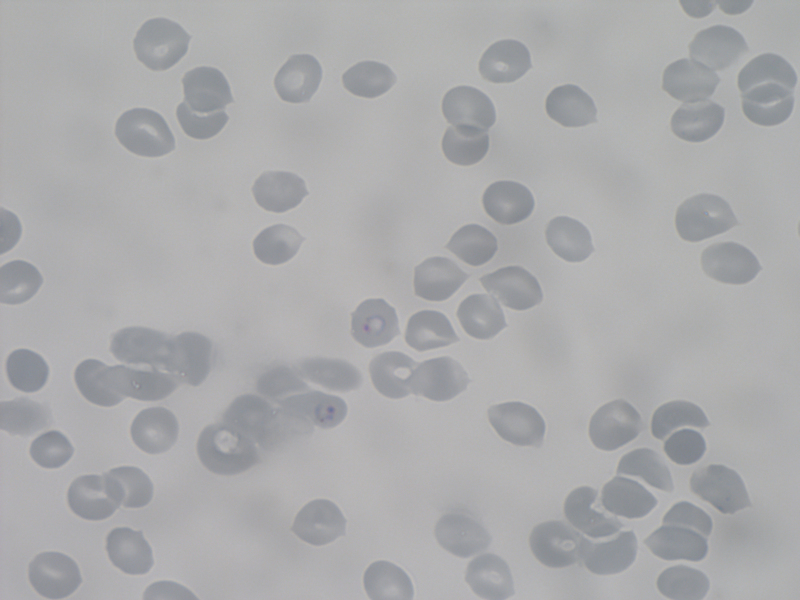
\includegraphics[width=\textwidth]{../data/natural001.jpg}
      \caption{Red blood cells infected with Malaria parasites (\emph{rbc}), $1600
        \times 1200$ pixels.}
      \label{fig:nat-a}
    \end{subfigure}
    ~
    \begin{subfigure}{0.3\textwidth}
      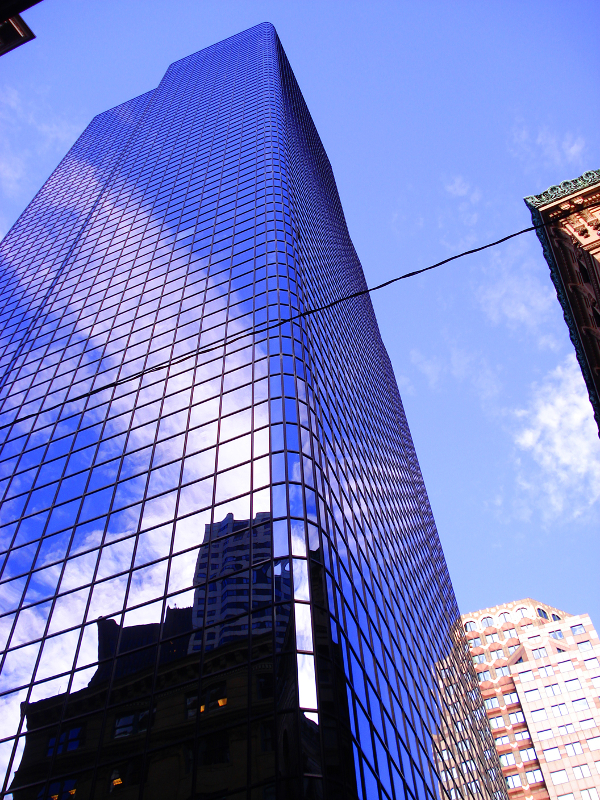
\includegraphics[width=\textwidth]{../data/natural002.jpg}
      \caption{Facade of an office building (\emph{facade}), $600 \times 800$ pixels.}
      \label{fig:nat-b}
    \end{subfigure}
    ~
    \begin{subfigure}{0.3\textwidth}
      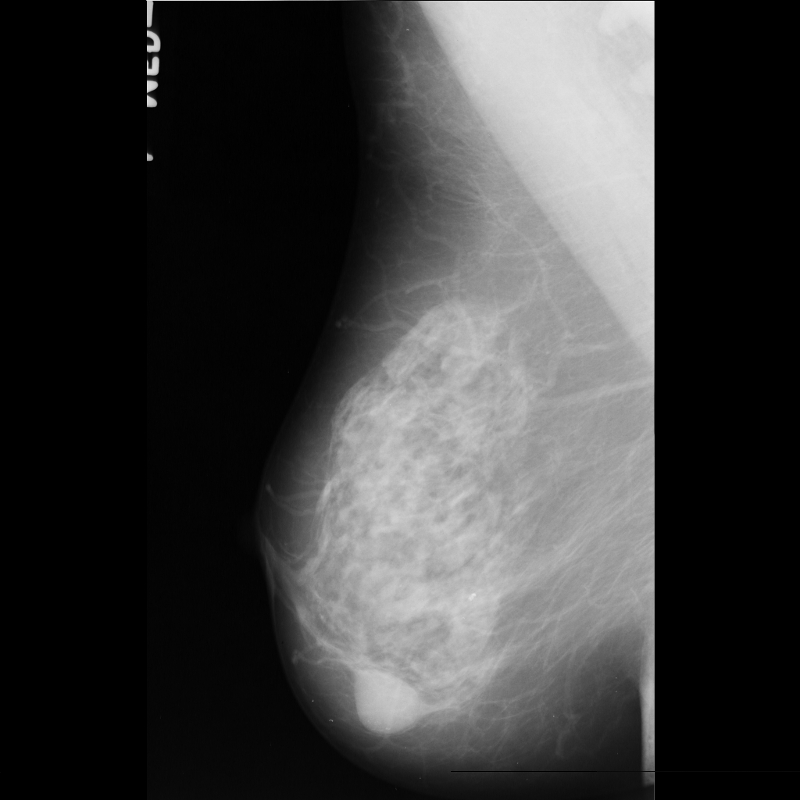
\includegraphics[width=\textwidth]{../data/natural003.jpg}
      \caption{Mammography scan (\emph{mammo}), $800 \times 800$ pixels.}
      \label{fig:nat-c}
    \end{subfigure}
  } % makebox

  \caption[Natural input images for area-opening experiments.]{Natural input
    images for area-opening experiments. The images represent different
    real-life use cases of morphological area opening.}
  \label{fig:nat}
\end{figure}

\begin{figure}
  \centering
  \plotsingle
  {\natone\ms\opt}
  {Results for \emph{rbc}.}
  {nat-results-a}

  \plotrow
  {\nattwo\ms\opt|pixel}
  {Results for \emph{facade}.}
  {nat-results-b}
  {\natthree\ms\opt|pixel}
  {Results for \emph{mammo}.}
  {nat-results-c}
  \caption[Execution time in milliseconds for natural images using optimistic
  union-find.]{Execution time in milliseconds for natural images using
    optimistic union-find. It becomes clear that there is a lower bound on the
    image size with regard to speedup. Also, there is an upper bound on number
    of threads, as in most cases, the performance declines around eight
    threads.}
  \label{fig:nat-results}
\end{figure}

To validate the results against real life input, we will concern three realistic
cases of natural images, which can be analyzed using morphological area opening
in various forms. The images are displayed in figure~\ref{fig:nat}. Due to being
captured by different means, the dimensions of these images vary. All images
were converted to 8-bit gray-scale.

Figure~\ref{fig:nat-a} shows a blood sample Malaria parasites
(\emph{rbc}). The photography in figure~\ref{fig:nat-b} shows the facade of an
office building (\emph{facade}). In figure~\ref{fig:nat-c}, we see a mammography
scan of a female breast (\emph{mammo}), which has been obtained from \emph{The
  Mammographic Image Analysis Society digital mammogram database}
\cite{Suckling1994Mammographic}.

The benchmark results for the natural images are displayed in
figure~\ref{fig:nat-results}. It is easy to see that the behavior of the
algorithms on natural images closely resembles the results obtained on synthetic
images. These plots also make it very clear, that there is a lower bound on the
image size, that needs to be taken into account, in order to gain any
performance increase by using parallel area opening.

Also, there is an upper bound on the number of threads with regard to
performance in the majority of cases. We see in both figures that the, already
encountered, upper bound on threads seems to be a pattern. The performance
declines around eight threads (see again figures~\ref{fig:nat-results-b} and
\ref{fig:nat-results-c}). This might be due to a larger number objects crossing
sub-image borders on natural images.

The results for \emph{rbc} (figure~\ref{fig:nat-results-a}) closely resemble the
results for fine grained synthetic noise images,
i.e. figure~\ref{fig:hypothesis-2-a}. The performance on \emph{facade} and
\emph{mammo} (figures~\ref{fig:nat-results-b} and \ref{fig:nat-results-c}) is
comparable to the results shown in figure~\ref{fig:hypothesis-2-b} with a twist:
the natural input images have smaller dimensions and the algorithms, at no time,
outperform sequential area opening. We can conclude that this is due to the
input image size and that it therefore does not pay off to filter small images
(i.e. $800 \times 600$ pixels) using parallel area opening.

\subsection{Scaling Behavior for $\lambda$}
\label{sec:experiments-ao-scale}

There is one more parameter, which we did not yet address. The size of $\lambda$
has an effect on the size of connected components: it is the upper bound on size
for non-level pixel components (see section~\ref{sec:morphology-area-opening})
and therefore potentially influences lock contention. If the structure of the
image only allows for components smaller than $\lambda$, or, if the image
exhibits a large number of flat level components, its effect is countered.

Experiments on \emph{noise-fine} suggest that practical values of $\lambda$ do
not have any immediate effect on sub-image filtering algorithms (see results in
figure~\ref{fig:scale-results}). Also, he sequential base-line does not change
with increased $\lambda$. This is actually true for differently structured
images as well, if we take the results presented in
section~\ref{sec:experiments-ao-results} into account.

The parallel algorithms do not behave equally for increased values of
$\lambda$. There is a slight performance drop exhibited by
\emph{block-counting}. Since its performance already is poor, the changes are
barely noticeable. Different so for line-based filtering. By comparing
figure~\ref{fig:scale-results-6000} to figure~\ref{fig:scale-results-9000}, it
becomes obvious that the line-based algorithm does indeed suffer from increased
$\lambda$. The sub-image filtering algorithms, however, exhibit constant
performance for increased $\lambda$, which is a clear advantage.

We can conclude that, for practical values of $\lambda$, its effect on the
performance of the sub-image algorithms is negligible in comparison to image
structure. This is supported by the experimental results presented by
\citet{Meijster2002Comparison}, which indicate no dependency of the performance
of union-find area opening in relation to $\lambda$. Therefore, optimistic
sub-image filtering with thread-local sorting is not only the fastest, but also
the most robust parallel algorithm for area opening.

\begin{figure}
  \centering
  \plotrow{\synththreeb\ms\opt}{}{scale-results-6000}{\synththreec\ms\opt}{}{scale-results-9000}
  \caption[Benchmark results for \emph{noise-fine} and increasing $\lambda$
  using optimistic union-find.]{Benchmark results for \emph{noise-fine} and
    increasing $\lambda$ using optimistic union-find. Sub-image filtering
    algorithms are not affected by increasing values of $\lambda$, but
    line-based and shared-sorting variants react with declining performance.}
  \label{fig:scale-results}
\end{figure}

%%% Local Variables:
%%% mode: latex
%%% TeX-master: "main"
%%% End:
